\section{Baseline Comparison: Supplementary Details}

This section provides supplementary evidence for the baseline comparison in \S\ref{sec:eval-comparison}. We first summarize budget alignment, engineering implementation details, and a capability overview in \S\ref{sec:appendix-comp-budget}, then supplement robustness evidence for triage and gating comparisons in \S\ref{sec:appendix-comp-triage} and \S\ref{sec:appendix-comp-gating}, respectively; complete threshold sweep tables are provided at the end for reference.
Figure~\ref{fig:b3_bucket_tree} illustrates the hierarchical bucket tree structure of B3 for reference in subsequent discussions.
Table~\ref{tab:c5-2} summarizes the capability comparison of all methods across the four dimensions of triage, gating, sizing, and control-plane cost.



\begin{table*}[!thbp]
\centering
\small
\begin{tabular}{lllll}
\toprule
Dimension & SCOUT & B2 (CountSketch ranking) & B3 (bucket tree) & B1 (checksum) \\
\midrule
\textbf{Triage feasible region} & \shortstack{Wide (still usable at \\ high \texttt{S/B} + low \texttt{ratio})} & \shortstack{Narrow (extensive \\ N/A at low \texttt{ratio})} & \shortstack{Narrow (step-wise \\ inflation from leaf \\ bucket expansion)} & \shortstack{Degrades linearly \\ with \texttt{S/B} (no ranking)} \\
\midrule
\textbf{Gating discriminability} & \shortstack{$\checkmark$ (viable operating \\ point exists)} & \shortstack{$\times$ (no viable \\ trade-off)} & \shortstack{$\times$ (no viable \\ trade-off)} & \shortstack{N/A \\ (no shape signal)} \\
\midrule
\textbf{Sizing} & \shortstack{$\checkmark$ \\ (validated in \S\ref{sec:eval-dedrift})} & \shortstack{$\times$ \\ (per-segment ranking only)} & \shortstack{Limited (bucket-level \\ energy, not segment-level)} & \shortstack{$\times$ \\ (count only)} \\
\midrule
\textbf{Control-plane cost} & \shortstack{$O(1)$ \\ (fixed $\sim$512 KiB)} & \shortstack{$O(1)$ \\ (same order)} & \shortstack{$O(1)$ \\ (same order)} & \shortstack{$O(P)$ ($\sim$tens of MB \\ at $P=10^6$)} \\
\midrule
\shortstack{\textbf{Can scaling} \\ \textbf{mitigate failure?}} & \shortstack{Partially \\ ($V$ is the primary knob)} & \shortstack{Limited (core failure \\ region remains unreachable)} & \shortstack{Limited (bounded by \\ structural inflation)} & N/A \\
\bottomrule
\end{tabular}
\caption{Capability matrix (same budget, single-round probe): comparison across triage, gating, sizing, and control-plane cost.}
\label{tab:c5-2}
\end{table*}


\subsection{Budget Alignment and Capability Overview}
\label{sec:appendix-comp-budget}

\paragraph{Budget conversion}
Table~\ref{tab:c5-0} lists the digest budget conversion for each method in the triage comparison; Table~\ref{tab:c5-gating-budget} provides the digest budget alignment at the $\sim$768\,KiB tier for the gating comparison.

\begin{table*}[!thbp]
\centering
\small
\begin{tabular}{lllr}
\toprule
Method & Key parameters & Memory formula & Estimated size \\
\midrule
SCOUT & \texttt{V=2, L=2048, m0=32, k=3, W=2} & $V\cdot L\cdot m_0\cdot 4$ bytes &  $\sim$512 KiB \\
B2-w11k & \texttt{views=2, rows=3, width=11264} & $\text{views}\cdot \text{rows}\cdot \text{width}\cdot 8$ bytes & $\sim$528 KiB \\
B2-w22k & \texttt{views=2, rows=3, width=22528} & same as above ($2\times$ width) & $\sim$1.03 MiB \\
B3-c4 & \texttt{b=8, depth=5, cells\_per\_bucket=4} & $\text{total\_nodes}\cdot m\cdot 4$ bytes &  $\sim$585 KiB \\
B3-c8 & \texttt{b=8, depth=5, cells\_per\_bucket=8} & same as above ($2\times$ cells) & $\sim$1.14 MiB \\
\bottomrule
\end{tabular}
\caption{Digest budget alignment for triage comparison (primary configuration $\sim$512\,KiB; B2-w22k and B3-c8 serve as $2\times$ memory controls).}
\label{tab:c5-0}
\end{table*}




\begin{table}[!thbp]
\centering
\small
\setlength{\tabcolsep}{2pt}
\begin{tabular}{@{}llc@{}}
\toprule
Method & Key parameters & \shortstack[c]{Estimated\\size} \\
\midrule
SCOUT & \shortstack[l]{\texttt{V=3, L=2048, m0=32, k=2, W=3}} & $\sim$768 KiB \\
B2 & \shortstack[l]{\texttt{views=3, rows=3, width=11264, K=2000}} & $\sim$792 KiB \\
B3 & \shortstack[l]{\texttt{b=8,depth=5,k=3,t=8,cells\_per\_bucket=6} } & $\sim$878 KiB \\
\bottomrule
\end{tabular}
\caption{Digest budget alignment at the $\sim$768\,KiB tier (gating comparison).}
\label{tab:c5-gating-budget}
\end{table}

\paragraph{Accumulator width and budget fairness}

B2 uses int64 accumulators following common industrial implementations (libraries such as Apache DataSketches and Twitter Algebird default to 64-bit accumulators). This choice is motivated by two engineering considerations. First, during the local build phase (before differencing), the single-side digest must accumulate raw counts over a full scan; when data volume reaches $10^9$ and significant skew is present, a wider accumulator provides the necessary safety margin. Second, the decoding phase involves squaring accumulators and computing concentration statistics, where int64 avoids overflow risk in intermediate steps.
In contrast, SCOUT's two-level mapping restricts each key's updates to the $W \cdot m_0$ cells within its window; the worst-case per-cell accumulation is bounded by the window capacity, which falls well below the int32 limit under typical parameters. Under skewed workloads (e.g., YCSB Zipfian), hot segments concentrate large numbers of keys into the same window of $W \cdot m_0$ cells. Taking the worst case of $10^9$ records, $k{=}3$, $W \cdot m_0 = 4 \times 32 = 128$, the per-cell load is approximately $10^9 \times 3 / 128 \approx 2.3 \times 10^7$, well below the int32 limit (${\sim}2.1 \times 10^9$), providing ample safety margin.

It should be noted that B2's use of int64 yields roughly half the number of counters compared to an int32 scheme at the same budget. To rule out this discrepancy as a confound, B2's $2\times$ memory control (B2-w22k) matches the counter count of the int32 baseline configuration.


\begin{figure}[!htbp]
  \centering
  \resizebox{0.98\linewidth}{!}{%
  \begin{tikzpicture}[
      font=\small,
      bucket/.style={circle,draw=gray!35,minimum size=7mm,inner sep=0pt,fill=white},
      bucketSel/.style={circle,draw=blue!70!black,very thick,minimum size=7mm,inner sep=0pt,fill=blue!8},
      edge/.style={-Latex,thick,draw=gray!30},
      edgeSel/.style={-Latex,very thick,draw=blue!70!black},
      box/.style={draw=gray!60,rounded corners,fill=gray!5},
      seg/.style={draw,minimum size=4.2mm,inner sep=0pt,rounded corners=0.5pt},
      segClean/.style={seg,fill=gray!25,draw=gray!45},
      segDirty/.style={seg,fill=red!70,draw=red!80!black},
      note/.style={align=left},
      brace/.style={decorate,decoration={brace,amplitude=4pt}}
    ]

    % --- Hierarchical bucket tree ---
    \node[bucket] (root) {root};
    \node[above=3mm of root, font=\bfseries] {Update \& Drill-down};

    \node[bucket,below=10mm of root] (l1m) {};
    \node[bucket,below left=10mm and 18mm of root] (l1l) {};
    \node[bucket,below right=10mm and 18mm of root] (l1r) {};

    \draw[edge] (root) -- (l1l);
    \draw[edge] (root) -- (l1m);
    \draw[edge] (root) -- (l1r);

    \node[bucket,below=10mm of l1m] (l2m) {};
    \node[bucket,below left=10mm and 12mm of l1m] (l2l) {};
    \node[bucket,below right=10mm and 12mm of l1m] (l2r) {};

    \draw[edge] (l1m) -- (l2l);
    \draw[edge] (l1m) -- (l2m);
    \draw[edge] (l1m) -- (l2r);

    % Selected drill-down path
    \node[bucketSel] (l1ms) at (l1m) {top-$t$};
    \node[bucketSel] (l2ms) at (l2m) {leaf};
    \draw[edgeSel] (root) -- (l1ms);
    \draw[edgeSel] (l1ms) -- (l2ms);

    % --- Visualize "collateral expansion" at the selected leaf ---
    % Reduced box width (44mm) and increased distance from leaf node above to accommodate text
    \node[box,below=15mm of l2ms,minimum width=44mm,minimum height=20mm] (bucketbox) {};
    
    % Attach text to the arrow side to avoid overlapping with the box
    \draw[edgeSel] (l2ms) -- (bucketbox.north) node[midway, right=2mm, font=\bfseries] {Expand selected bucket};

    % Center the internal segments
    \coordinate (center) at (bucketbox.center);
    % 5 columns x 2 rows grid, dynamically offset from center point
    \foreach \i [evaluate=\i as \xoff using (\i-2)*5.5] in {0,...,4} {
      \foreach \j [evaluate=\j as \yoff using (0.5-\j)*5.5] in {0,1} {
        \node[segClean] at ($(center)+(\xoff mm, \yoff mm)$) {};
      }
    }
    % Draw a conspicuous dirty segment (placed at i=1, j=0 position, i.e., upper-left side, appears natural)
    \node[segDirty] at ($(center)+(-5.5 mm, 2.75 mm)$) {};

    \node[below=1.5mm of bucketbox.south, note]
      {\textbf{1}~dirty segment mixed with \textbf{many}~clean ones};

    % --- Cost jump annotation ---
    % Draw right brace
    \draw[brace,thick,draw=red!75!black] ($(bucketbox.north east)+(1.5mm,0mm)$) -- ($(bucketbox.south east)+(1.5mm,0mm)$);
    
    % Draw staircase red line starting from right of brace (extends right 12mm)
    \coordinate (stair_start) at ($(bucketbox.east)+(3.5mm,-3mm)$);
    \draw[thick,draw=red!75!black] (stair_start) -- ++(4mm,0) -- ++(0,2.5mm) -- ++(4mm,0) -- ++(0,2.5mm) -- ++(4mm,0) coordinate (stair_end);
    
    % Text strictly aligned to the right of staircase endpoint, completely prevent overlap
    \node[anchor=west, note] at ($(stair_end)+(1mm, -2.5mm)$) {\textbf{Cost jump}\\$+P/b^{d}$ candidates};

    % Weaken unselected branches
    \foreach \n in {l1l,l1r,l2l,l2r} {
      \node[bucket,draw=gray!25,text=gray!60] at (\n) {};
    }

  \end{tikzpicture}%
  }
  \caption{B3 (hierarchical bucket tree) baseline: segments are mapped to leaf nodes of a fixed tree ($b{=}3, d{=}2$ in this example). During reconciliation, the probe drills down from root to leaves by selecting high-score buckets at each level. Once a leaf bucket is selected, \emph{all} segments in that bucket---including the many clean ones---must be expanded as candidates, causing a step-wise cost jump.}
  \label{fig:b3_bucket_tree}
\end{figure}

\subsection{Triage Robustness}
\label{sec:appendix-comp-triage}

\subsubsection{Scaling Control and Failure Region}

\begin{table*}[!thbp]
\centering
\small
\begin{tabular}{rcllll}
\toprule
\texttt{S/B} & \texttt{ratio} & SCOUT & B2-w11k & B2-w22k & Notes \\
\midrule
10 & 200 & $\sim 2\times 10^{-4}$ & $\sim 1\times 10^{-4}$ & --- & \shortstack[l]{High-separability regime; \\ B2 achieves lower candidate budget }\\
\addlinespace
10 & 2--3 & $\sim 2\times 10^{-4}$--$7\times 10^{-4}$ & $\sim 2\times 10^{-3}$ & $\sim 1\times 10^{-3}$ & \shortstack[l]{Low-separability regime; SCOUT achieves \\  significantly lower candidate budget} \\
\addlinespace
100 & $\ge 5$ & $\sim 2\times 10^{-4}$ & $\sim 3\times 10^{-3}$--$1\times 10^{-2}$ & --- & \shortstack[l]{SCOUT quickly \\ returns to the low-cost region} \\
\addlinespace
100 & 2--3 & $\sim 7\times 10^{-4}$--degraded & $\sim 0.02$ (hitting cap) & $\sim 0.01$--0.02 & \shortstack[l]{Near the indistinguishability \\ boundary; both degrade} \\
\addlinespace
$\ge 1000$ & $\le 30$ & partially reachable & \textbf{N/A} & \shortstack[l]{few boundary \\ points reachable } & B2 exhibits a large failure surface \\
\addlinespace
$\ge 1000$ & $\ge 50$ & $\sim 10^{-3}$ & \textbf{N/A} & \textbf{N/A} & \shortstack[l]{SCOUT still viable;\\ B2 at $2\times$ memory remains unreachable }\\
\bottomrule
\end{tabular}
\caption{Threshold budget (\texttt{cand\_frac}) comparison at representative stress points. Rows correspond to pressure regions in Figure~\ref{fig:c5-b2-2x}; B2-w22k denotes B2's $2\times$ memory control; ``---'' indicates same order as the adjacent column.}
\label{tab:c5-triage-hints}
\end{table*}


\begin{figure*}[!thbp]
\centering
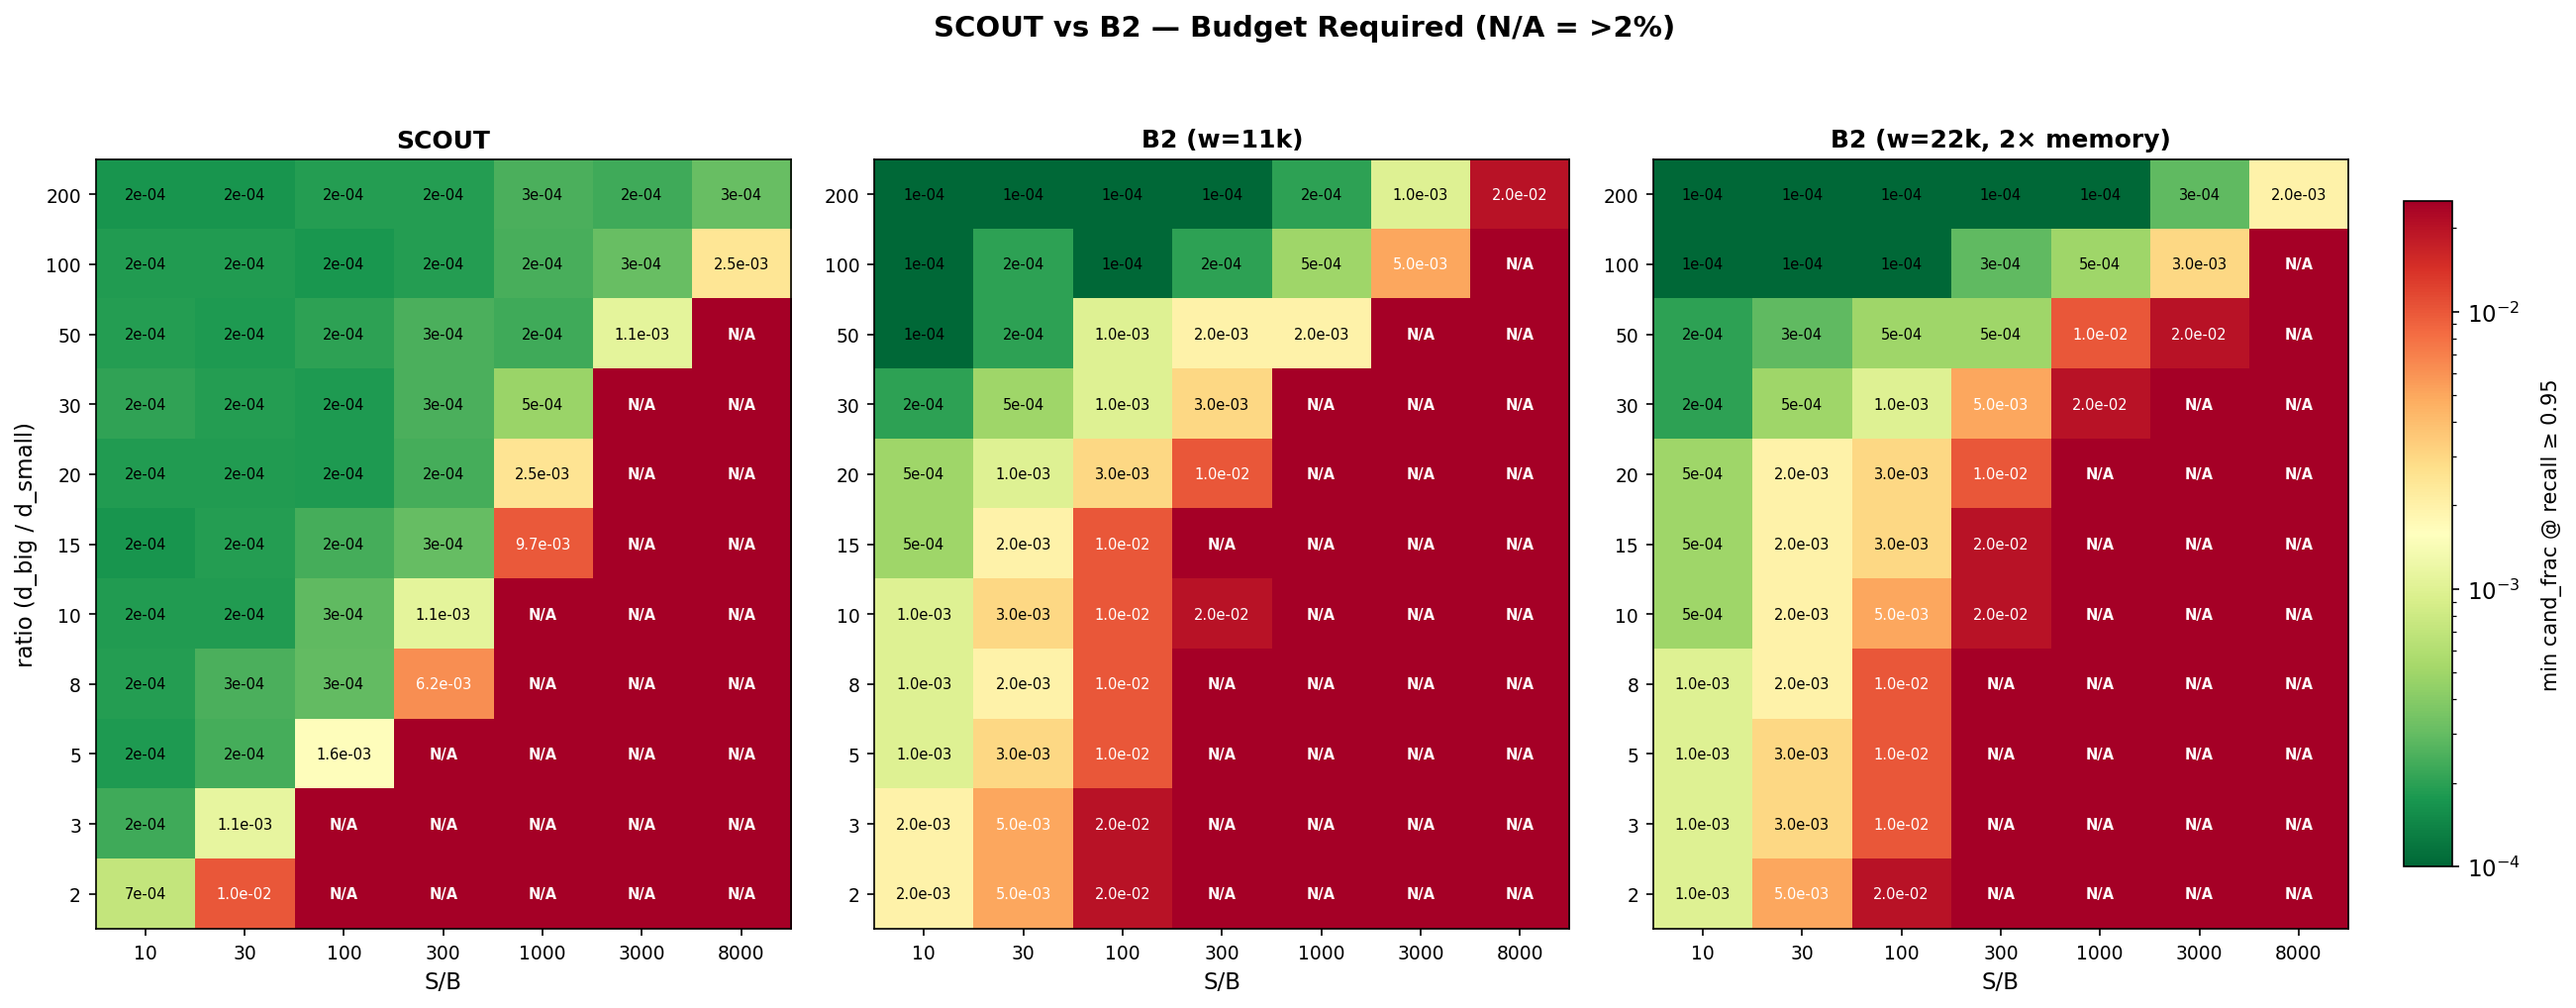
\includegraphics[width=0.9\linewidth]{figures/exp20v4_three_way_heatmap.png}
\caption{Three-way comparison heatmap after doubling B2's memory to $2\times$. Color scale matches Figure~\ref{fig:c5-1}; N/A indicates no feasible solution within the 2\% candidate budget cap.}
\label{fig:c5-b2-2x}
\end{figure*}

\begin{figure*}[!htbp]
\centering
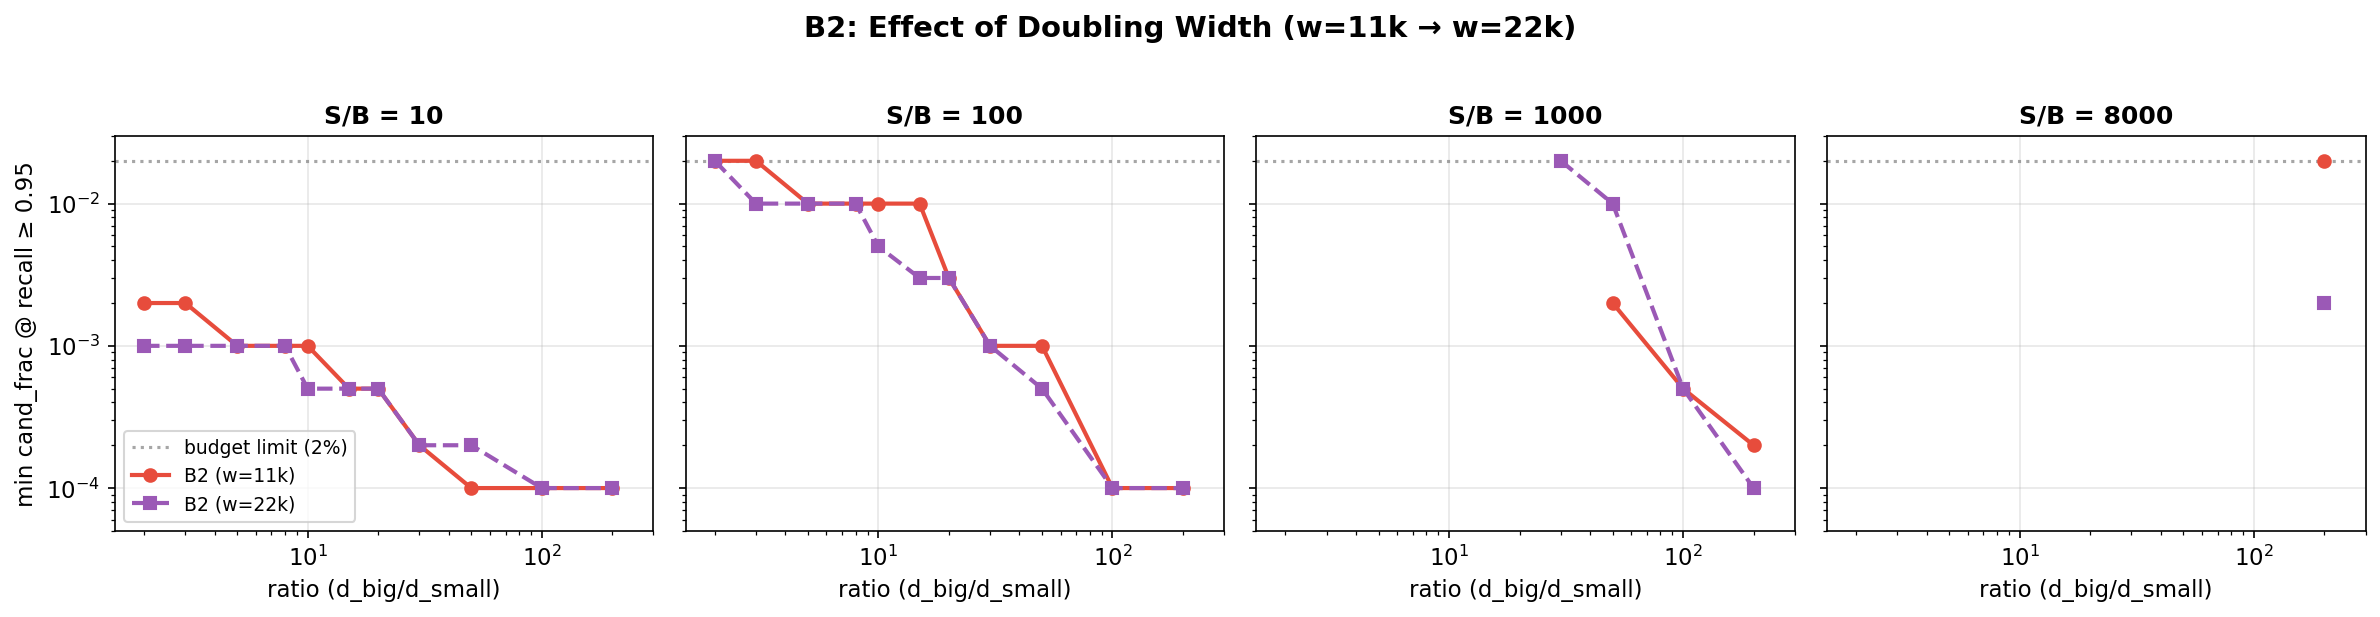
\includegraphics[width=0.9\linewidth]{figures/exp20v4_b2_width_comparison.png}
\caption{B2 scaling $2\times$ slice comparison. Each subplot fixes one \texttt{S/B}; dashed line marks the 2\% cap. In high-\texttt{S/B} slices, both width tiers approach or exceed the budget cap.}
\label{fig:c5-a2}
\end{figure*}

Figure~\ref{fig:c5-b2-2x} and Figure~\ref{fig:c5-a2} confirm this conclusion from two perspectives---the two-dimensional phase diagram and per-\texttt{S/B} slices, respectively: increasing the width produces visible budget reductions at lower \texttt{S/B} or higher \texttt{ratio}, but at very high \texttt{S/B} and very low \texttt{ratio}, both width tiers approach or exceed the 2\% candidate budget cap. B2's core failure region therefore persists after scaling up, consistent with the analysis in \S\ref{sec:eval-comparison}. Here B2-w11k denotes B2 with width 11{,}264, and B3-c4 denotes B3 with 4 cells per bucket. Numerical comparisons at representative stress points are provided in Supplement Table~\ref{tab:c5-triage-hints}.



\paragraph{Slice view: per-\texttt{S/B} threshold budget curves}

To visualize the boundary shape of the failure surface more intuitively, we present the two-dimensional phase diagram from Figure~\ref{fig:c5-1} as slice curves. Figure~\ref{fig:c5-2} fixes \texttt{S/B=1000} and shows each method's threshold budget as a function of \texttt{ratio}: B3-c4 falls below the 2\% cap only in the narrow interval $\texttt{ratio} \ge 20$; the $2\times$ memory control (B3-c8) extends the feasible region to $\texttt{ratio} \approx 8$--$15$, but lower \texttt{ratio} values remain N/A. Figure~\ref{fig:c5-a3} further unfolds \texttt{S/B} into multiple subplots, focusing on the SCOUT vs.\ B2 comparison: as \texttt{S/B} increases, B2's curve rapidly approaches the budget cap, while SCOUT maintains low cost over a wider range of \texttt{ratio}.

\begin{figure}[!htbp]
\centering
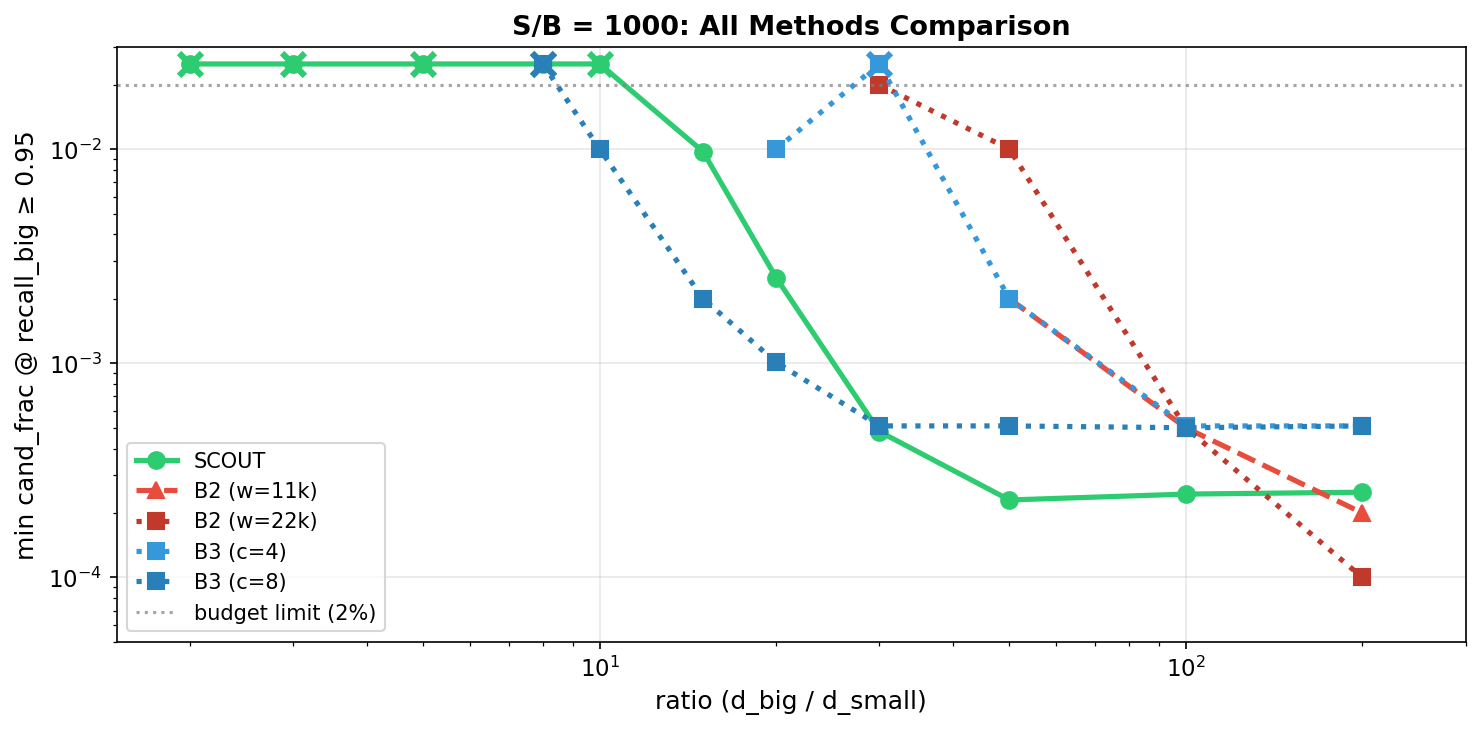
\includegraphics[width=0.9\linewidth]{figures/exp20v4_sb1000_all_methods.png}
\caption{Threshold budget curves for all methods at the \texttt{S/B=1000} slice. Lower is better; dashed line marks the 2\% cap.}
\label{fig:c5-2}
\end{figure}

\begin{figure*}[!htbp]
\centering
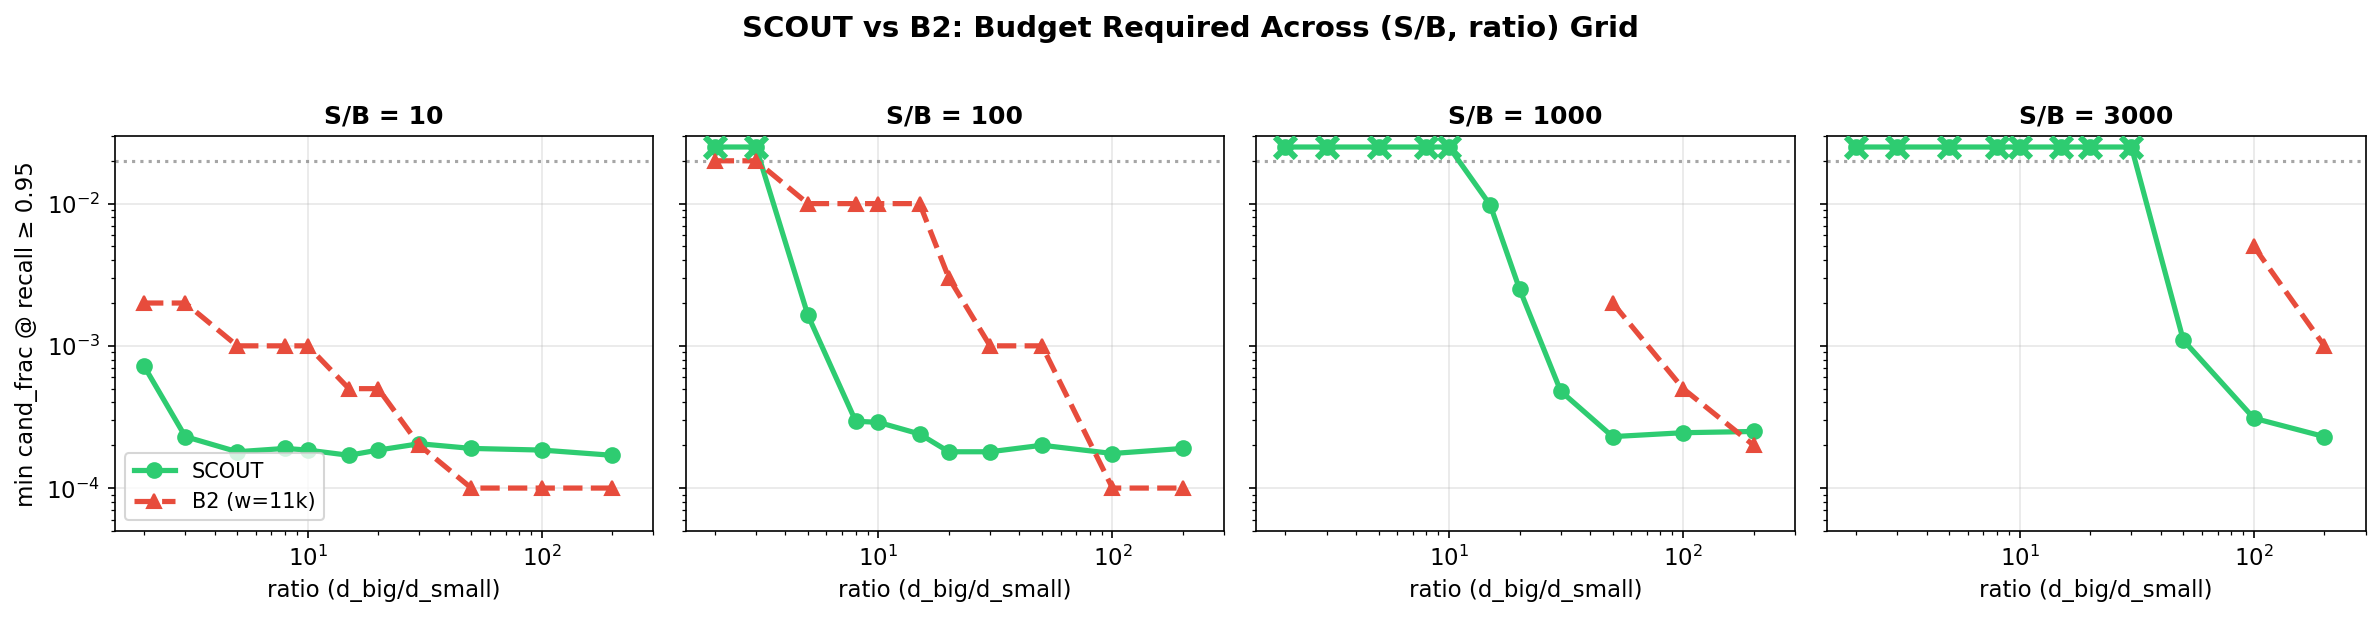
\includegraphics[width=0.9\linewidth]{figures/exp20v4_scout_vs_b2.png}
\caption{SCOUT vs.\ B2 per-\texttt{S/B} slice comparison. Each subplot fixes one \texttt{S/B};  Lower is better; dashed line marks the 2\% cap.}
\label{fig:c5-a3}
\end{figure*}

\subsubsection{Relative Threshold Budget Ratio}

To avoid misinterpretation from examining absolute threshold budgets alone, we additionally present the relative budget ratio (method / SCOUT). Figures~\ref{fig:c5-3} and~\ref{fig:c5-4} show the point-wise ratio for B2/SCOUT and B3-c4/SCOUT, respectively, where a higher ratio indicates that a larger candidate budget is needed to reach the same threshold; \texttt{FAIL} indicates the method has no feasible solution within $\le 2\%$ while SCOUT does, \texttt{ONLY} indicates only that method is feasible while SCOUT is not, and \texttt{N/A} indicates neither is feasible.

\begin{figure*}[!htbp]
\centering
\begin{minipage}[c]{0.48\linewidth}
  \centering
  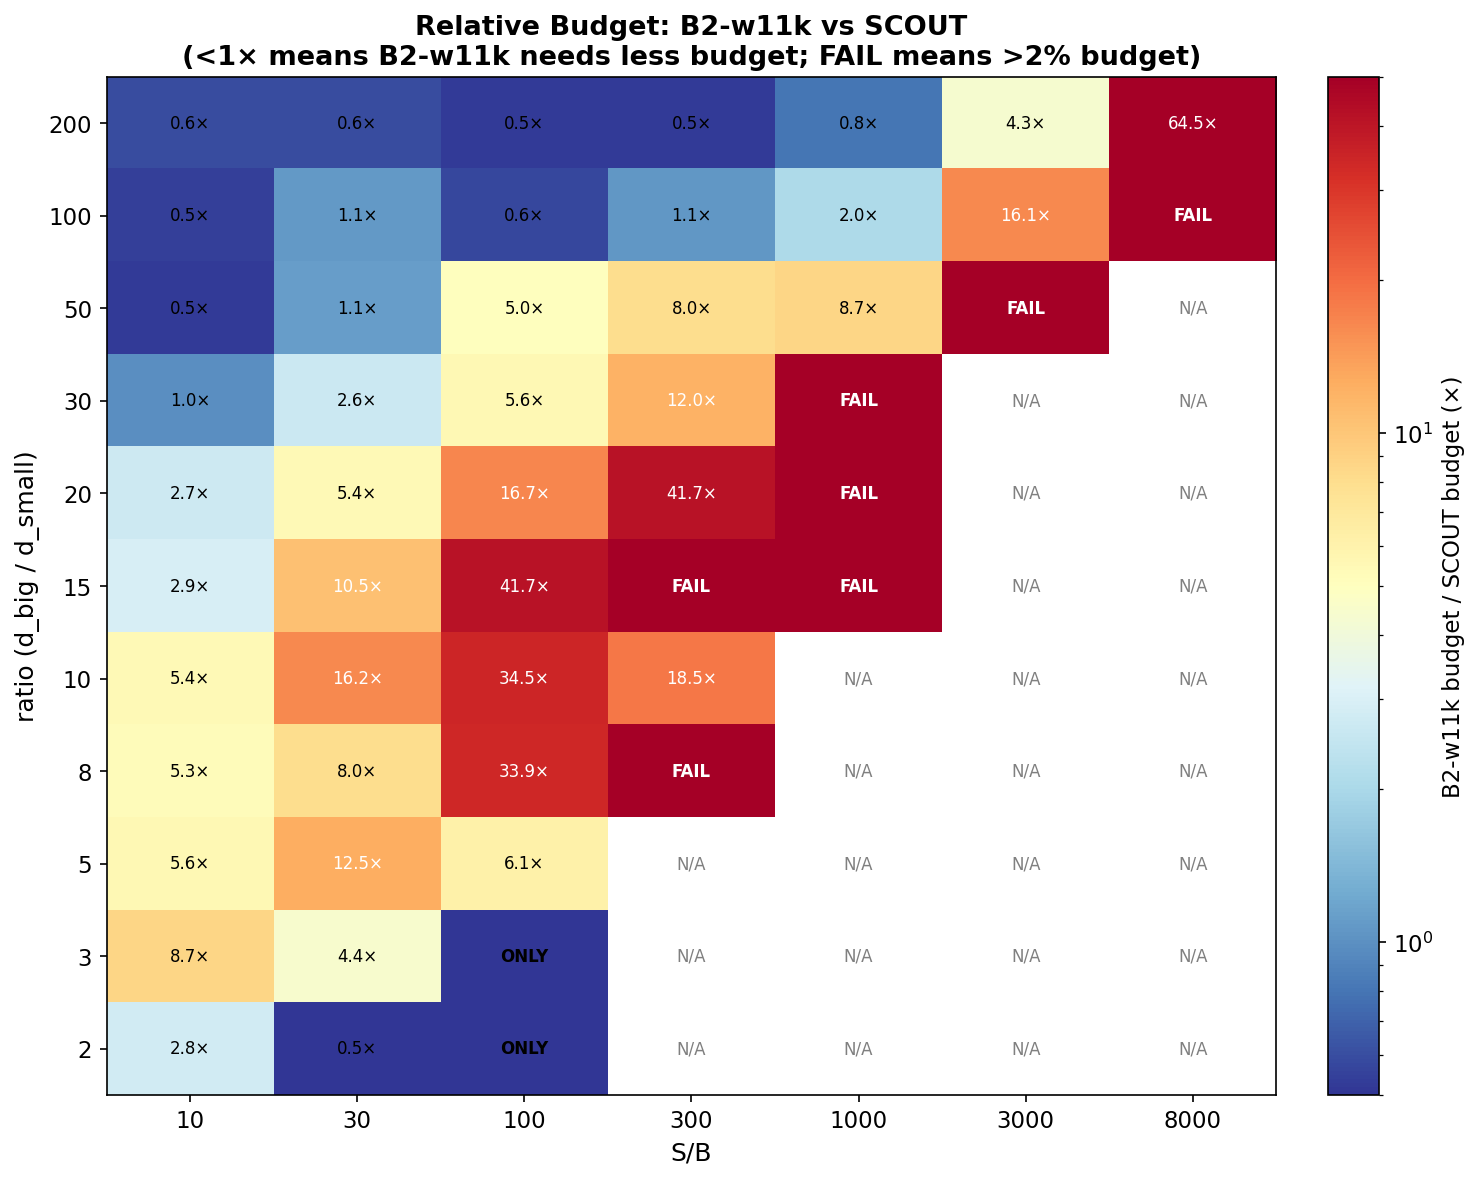
\includegraphics[width=\linewidth]{figures/exp20v4_budget_ratio_heatmap.png}
  \subcaption{B2 / SCOUT relative threshold budget ratio. \texttt{FAIL}: B2 has no feasible solution within the $\le 2\%$ cap while SCOUT does; \texttt{ONLY}: only B2 is feasible; \texttt{N/A}: neither is feasible.}
  \label{fig:c5-3}
\end{minipage}\hfill
\begin{minipage}[c]{0.48\linewidth}
  \centering
  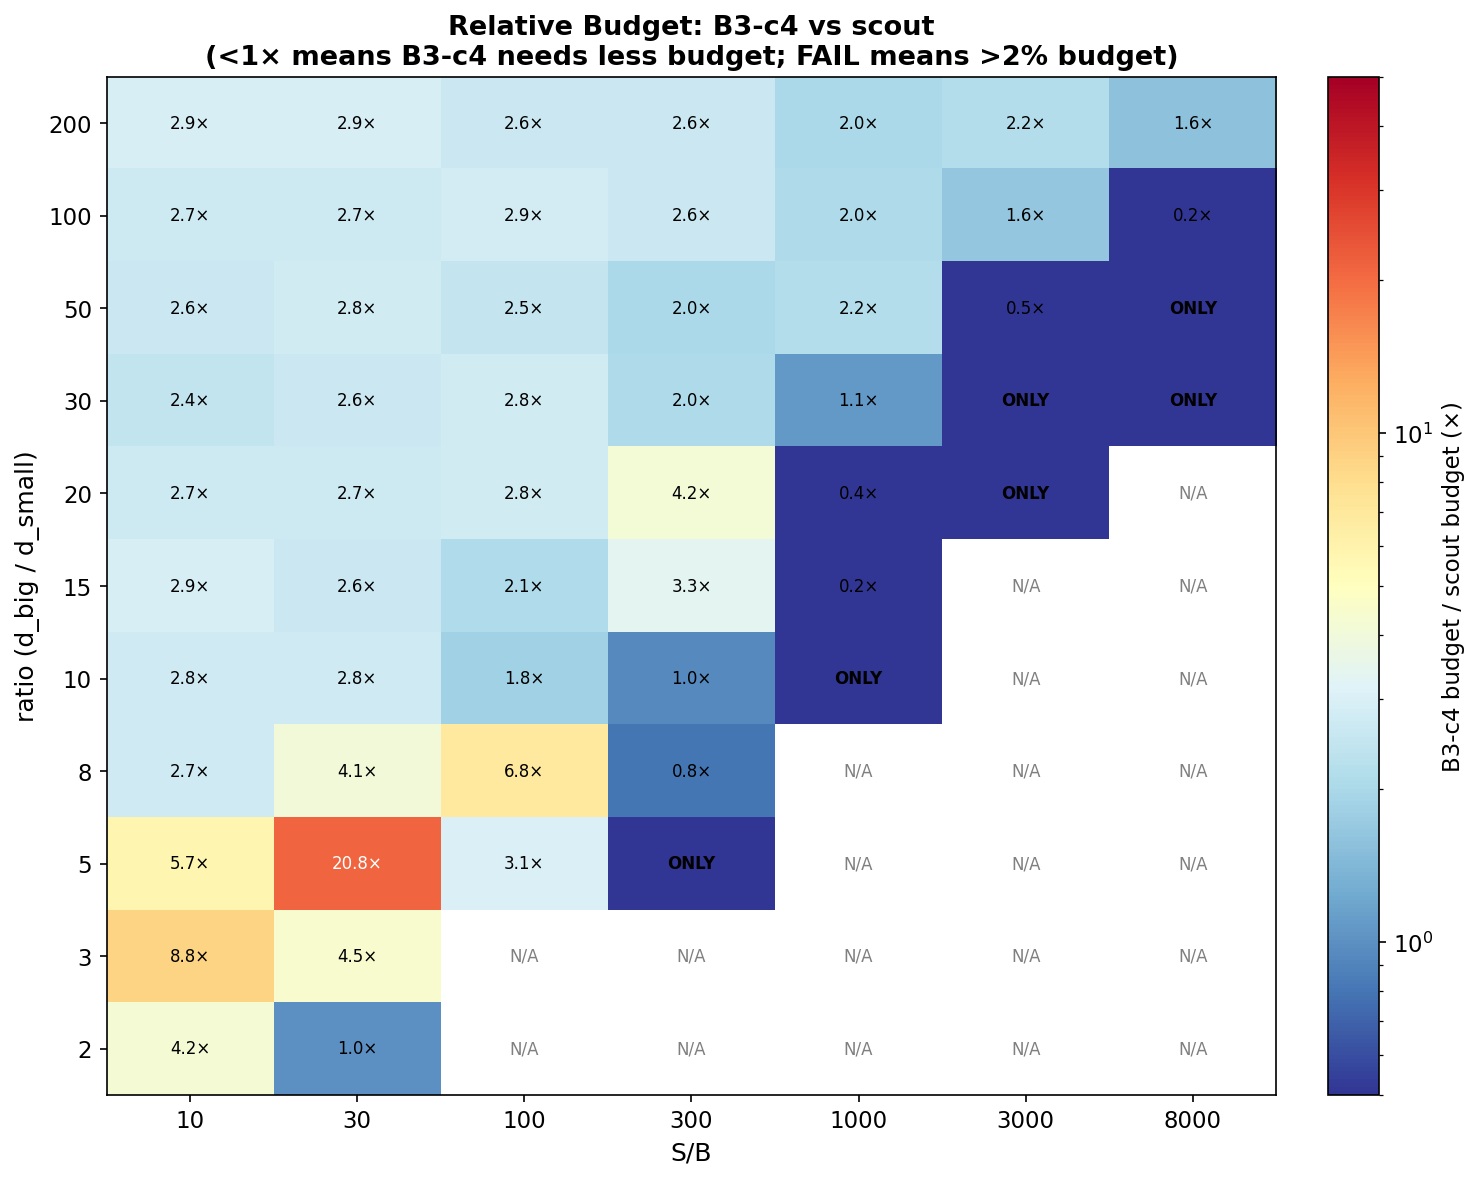
\includegraphics[width=\linewidth]{figures/exp20v4_b3c4_vs_scout_budget_ratio_heatmap.png}
  \subcaption{B3-c4 / SCOUT relative threshold budget ratio; \texttt{FAIL}/\texttt{ONLY}/\texttt{N/A} have the same meaning as in the left panel (with the comparison target replaced by B3-c4).}
  \label{fig:c5-4}
\end{minipage}
\caption{Relative threshold budget ratio heatmaps. Each cell shows the minimum \texttt{cand\_frac} needed to achieve $\texttt{median(recall\_big)} \ge 0.95$, relative to SCOUT ($>1$ indicates higher cost).}
\end{figure*}

\subsubsection{$B$ Ablation: $B=10 \to 100$}

The main results in \S\ref{sec:eval-comparison} are based on $B=10$ (i.e., 10 heavily dirty segments). To examine whether the triage advantage persists when the number of heavy faults $B$ increases, we raise $B$ from 10 to 100 and proportionally scale \texttt{total\_diff} ($200\text{K} \to 2\text{M}$) to keep the per-big-segment signal strength unchanged, so that performance changes are primarily driven by capacity pressure ($L/B$ decreasing from 204.8 to 20.48).
This change approaches the capacity threshold given by Eq.~\eqref{eq:capacity-threshold} in Supplement~\S\ref{sec:appendix-feasibility} ($L/B \gtrsim 16.3$ for $W{=}2$, $\alpha{=}1$); the widespread degradation at $B{=}100$ is therefore consistent with theoretical expectations.

The feasible-region changes on the shared grid (\texttt{S/B} $\in \{10, 30, 100, 300\}$ $\times$ \texttt{ratio} $\in \{2, 5, 10, 30, 50, 100, 200\}$ $= 28$ points) under the 2\% budget cap are shown in Table~\ref{tab:c5-a2}:

\begin{table}[!htbp]
\centering
\small
\begin{tabular}{lccc}
\toprule
Method & $B=10$ & $B=100$ & Degradation \\
\midrule
SCOUT & 89\% (25/28) & 64\% (18/28) & -25pp \\
\makecell[l]{B2(\texttt{w=11k})} & 93\% (26/28) & 50\% (14/28) & -43pp \\
\makecell[l]{B3(\texttt{c=4})} & 93\% (26/28) & 54\% (15/28) & -39pp \\
\bottomrule
\end{tabular}
\caption{$B$ ablation: feasible-region coverage change (2\% cap; 28-point grid).}
\label{tab:c5-a2}
\end{table}

All three methods degrade due to capacity pressure, but the degradation magnitudes differ (Table~\ref{tab:c5-a2}). Relaxing the candidate budget cap can partially recover the feasible regions of B2/B3; see the sensitivity analysis below.

\subsubsection{Sensitivity to the Candidate Budget Cap}


The main text uses 2\% as the candidate budget cap. A natural concern is whether this cap prematurely truncates the feasible regions of B2/B3. To address this, we relax the cap from 2\% to 5\% and 10\% under the $B{=}100$ scenario, and on the 35-point full grid count whether each method has an operating point satisfying the recall constraint within the given cap (Table~\ref{tab:c5-cap-sweep}).

\begin{table}[!thbp]
\centering
\small
\begin{tabular}{lccc}
\toprule
\makecell[l]{cap\\(\texttt{cand\_frac})} & SCOUT & B2 (w=11k) & B3 (c=4) \\
\midrule
0.02 & 57.1\% (20/35) & 40.0\% (14/35) & 45.7\% (16/35) \\
0.05 & 57.1\% (20/35) & 51.4\% (18/35) & 57.1\% (20/35) \\
0.10 & 62.9\% (22/35) & 60.0\% (21/35) & 71.4\% (25/35) \\
\bottomrule
\end{tabular}
\caption{Feasible-region coverage under candidate-budget caps ($B{=}100$, 35-point full grid).}
\label{tab:c5-cap-sweep}
\end{table}

Relaxing the cap does recover some of B2/B3's N/A points: for example, at the 5\% cap B3 matches SCOUT (both at 57.1\%), and at the 10\% cap B3 further improves to 71.4\%. However, matching coverage does not equate to matching end-to-end cost. Examining the color scales in Figure~\ref{fig:c5-cap5-heatmap} and Figure~\ref{fig:c5-cap10-heatmap}, the newly recovered points for B2/B3 have \texttt{cand\_frac} values that are generally close to the cap ceiling ($2{\times}10^{-2}$--$10^{-1}$), whereas SCOUT's typical operating points concentrate in the lower candidate range ($5{\times}10^{-3}$--$10^{-2}$). The 2\% cap therefore acts more as a practical downstream cap: it barely constrains SCOUT's natural operating range, but significantly affects whether B2/B3 remain feasible only near the cap ceiling at high-pressure stress points.

Furthermore, B3's recovery under relaxed caps is more pronounced, consistent with the discrete granularity of its leaf-bucket expansion: under a strict cap, step-wise jumps are more likely to hit the ceiling directly, while a relaxed cap more readily accommodates these jumps.

\begin{figure*}[!htbp]
\centering
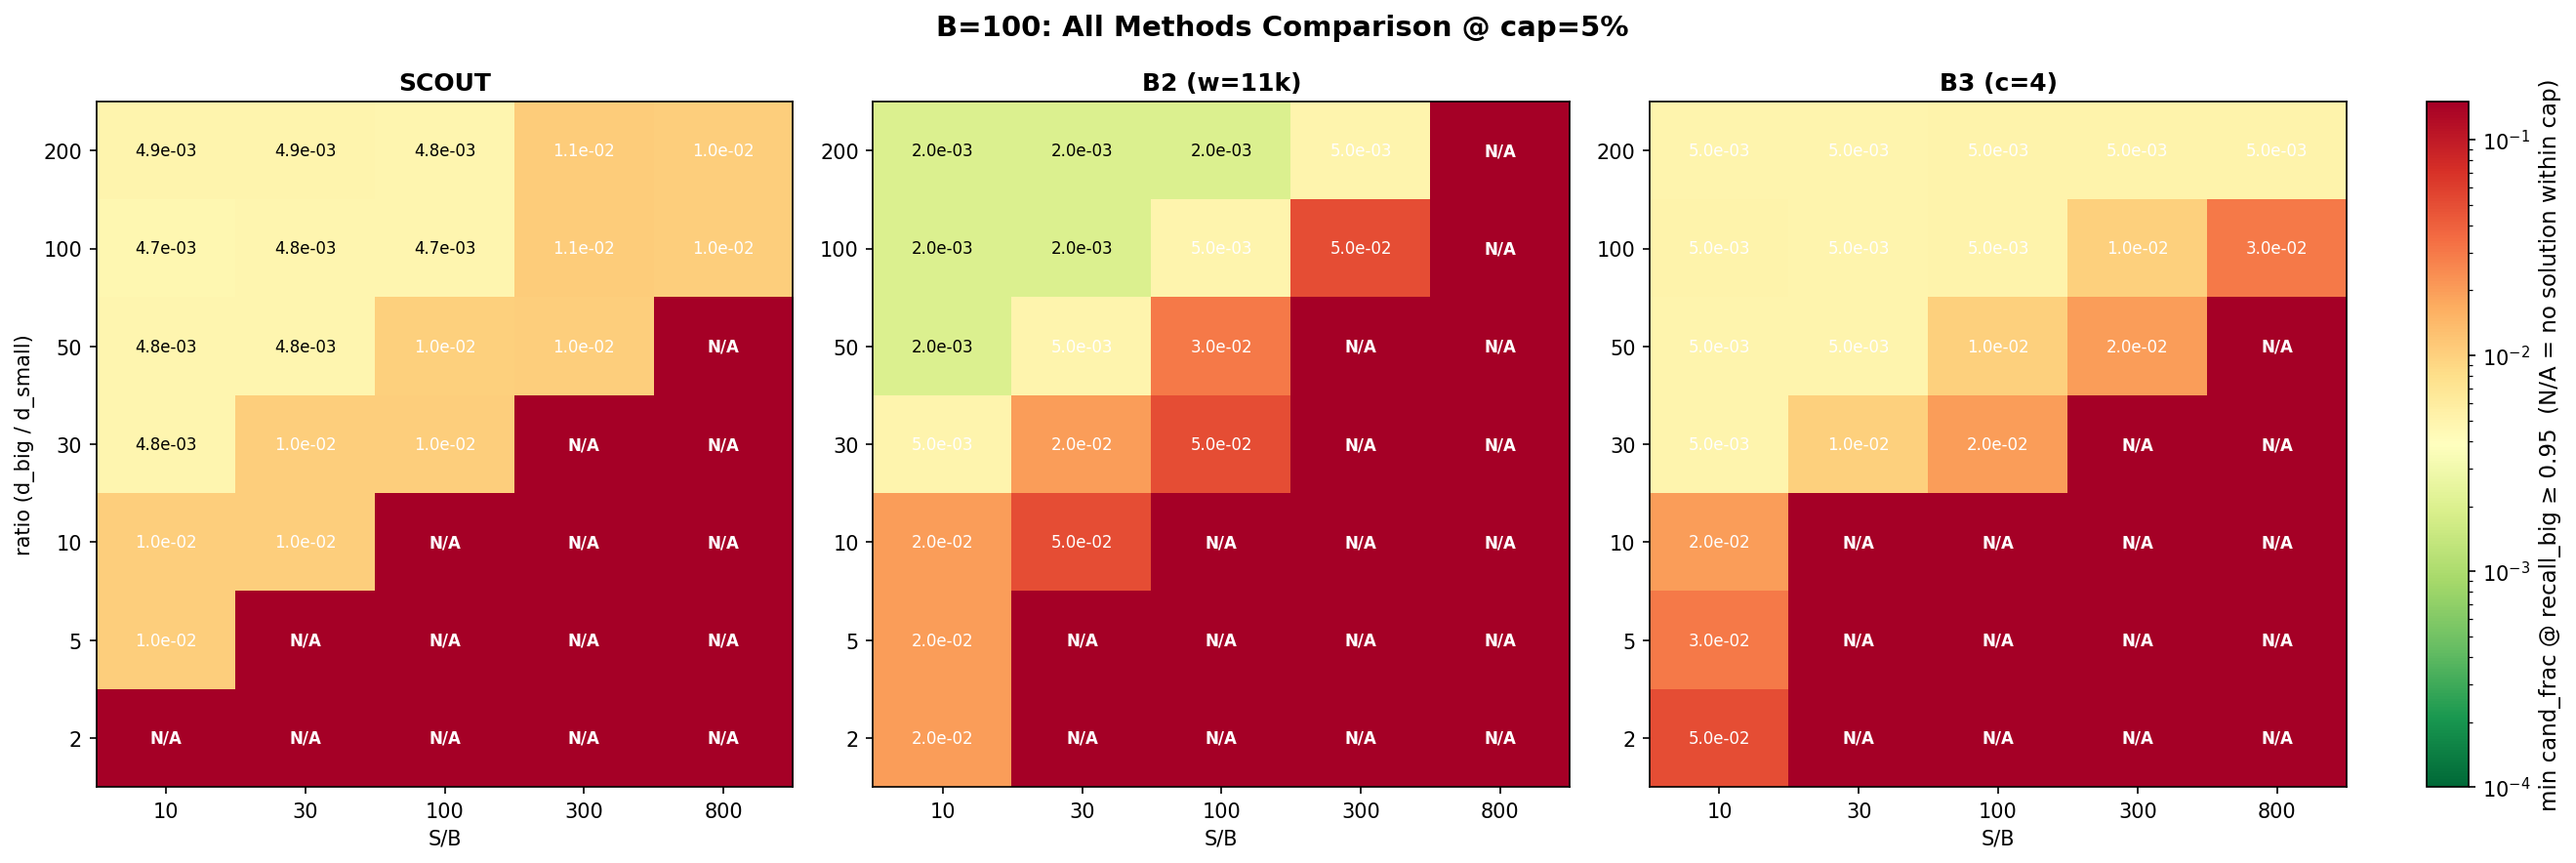
\includegraphics[width=0.95\linewidth]{figures/exp20v5b_all_methods_cap5.png}
\caption{Three-method heatmap at cap=5\% ($B{=}100$). Color scale matches Figure~\ref{fig:c5-1}; N/A indicates no feasible solution within the 5\% candidate budget.}
\label{fig:c5-cap5-heatmap}
\end{figure*}

\begin{figure*}[!htbp]
\centering
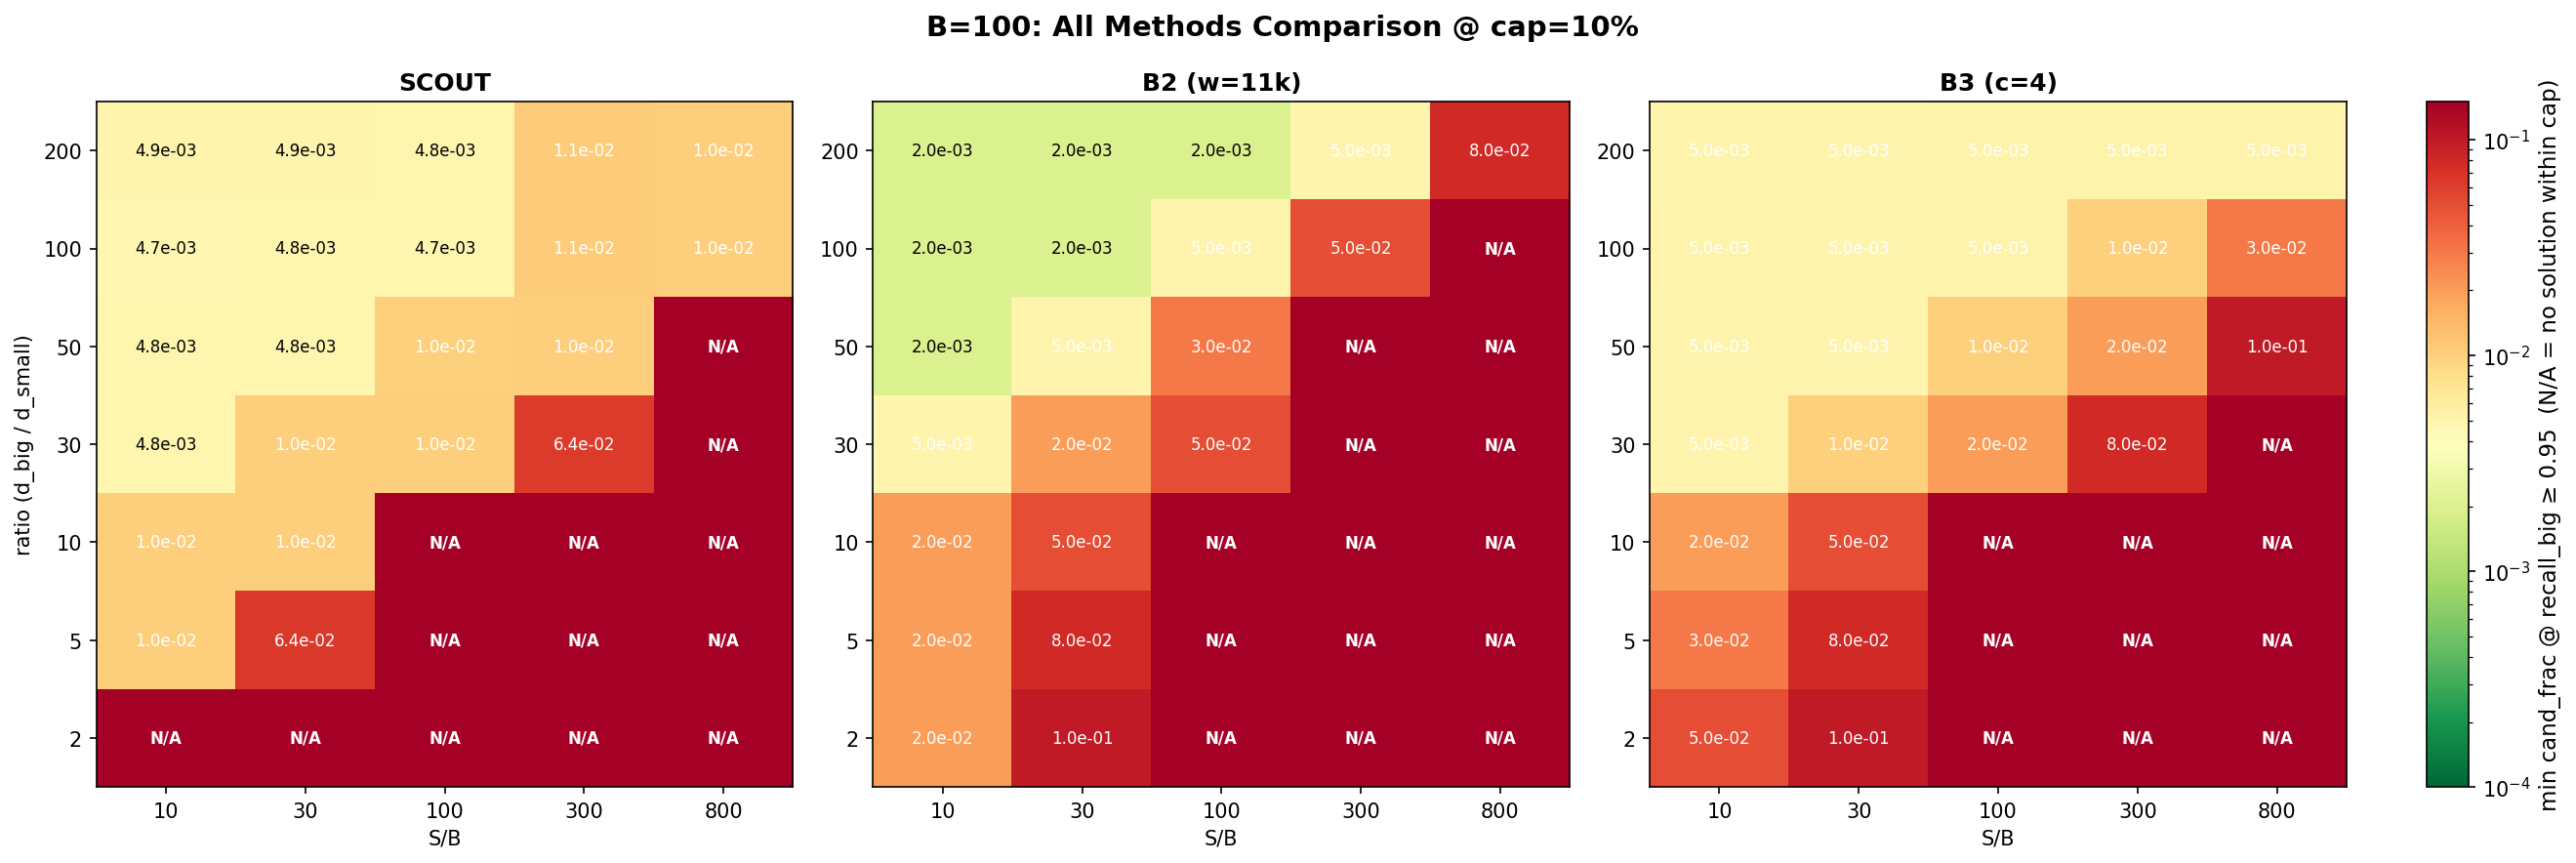
\includegraphics[width=0.95\linewidth]{figures/exp20v5b_all_methods_cap10.png}
\caption{Three-method heatmap at cap=10\% ($B{=}100$). Color scale matches Figure~\ref{fig:c5-1}; N/A indicates no feasible solution within the 10\% candidate budget.}
\label{fig:c5-cap10-heatmap}
\end{figure*}


\subsection{Gating Robustness}
\label{sec:appendix-comp-gating}

\subsubsection{Proxy Gating Score Definitions}
\label{sec:appendix-proxy-score}

For each method, we select a ``diffuseness'' proxy score consistent with its digest structure, and uniformly sweep the threshold $\tau_{\text{gating}}$ to report FAR--FRR and the decisive classification fraction. This section supplements the specific definitions and settings of each score.

SCOUT uses $K_{\text{eff}}/L$ from the section energy spectrum. B2 uses the head-mass residual $1-\rho_{\text{topK}}$, where
\[
  \rho_{\text{topK}}=\frac{\sum_{p\in \text{topK}}\hat{d}_p}{\sum_{p}\hat{d}_p}.
\]
The intuition is that concentrated faults are dominated by a few segments, so $\rho_{\text{topK}}\approx 1$ and $1-\rho_{\text{topK}}$ is close to 0; under diffuse discrepancies, the top-$K$ explains only a small fraction of total mass, and $1-\rho_{\text{topK}}$ rises. For consistency with the candidate budget criterion, we bind $K$ to the 2\% candidate cap. B3 uses the hierarchical expansion ratio
\[
  \text{expansion\_score}=\max_{\ell\in\{1,\dots,\text{depth}\}}\frac{\text{selected\_buckets}_\ell}{\text{total\_buckets}_\ell},
\]
with a fixed per-level selection strategy \texttt{top\_t\_per\_level=8}; the motivation is to align the score with B3's coarse-to-fine navigation process: the more diffuse the discrepancy, the more branches must be expanded to maintain recall.

We also considered alternative candidate scores. For B2, the Gini coefficient and top-$K$/top-$2K$ mass ratio are both based on the sorted estimated distribution and are highly collinear with $1-\rho_{\text{topK}}$, offering no qualitative improvement in discriminability. For B3, the average expansion ratio is diluted by the large number of unexpanded levels, losing the signal, while the discrete count of expanded levels produces more step-like FAR--FRR curves. The common limitation of these alternative scores is that B2 through hash aliasing and B3 through hierarchical aggregation both destroy spatial locality at the digest construction stage; any score based on such representations amounts to post-hoc inference on a representation that has already lost shape information, and the ceiling on discriminability is limited by the representation itself, not by the choice of score.

\subsubsection{Budget Control: $\sim$768 KiB Tier}

The main results in \S\ref{sec:eval-comp-gating} are based on the $\sim$512\,KiB tier, matching the triage budget. To verify that conclusions do not change with budget, this section adds a control at the $\sim$768\,KiB tier (SCOUT: \texttt{V=3/W=3}; B2: \texttt{views=3}; B3: \texttt{cells=6}); results are shown in Figure~\ref{fig:c5-5} and Table~\ref{tab:c5-1}. Conclusions are consistent across both budget tiers: SCOUT's optimal FAR is virtually unchanged ($\sim$0.038 vs.\ $\sim$0.039), while B2's $\texttt{FRR}=0.50$ plateau and B3's $\texttt{FAR}\approx 1.0$ phenomenon both persist regardless of budget, indicating that the failures originate from structural limitations.

\begin{figure}[!htbp]
\centering
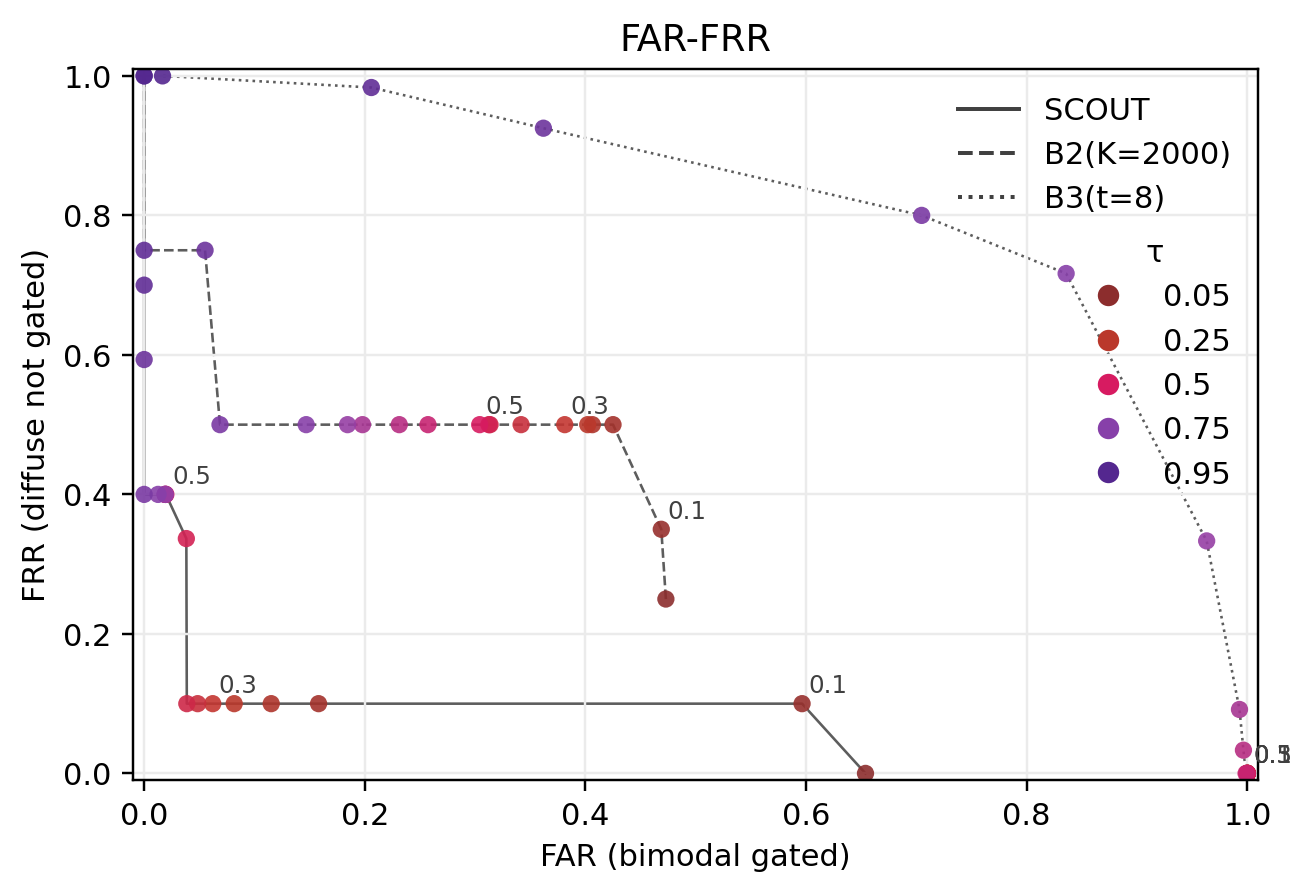
\includegraphics[width=0.99\linewidth]{figures/exp22v2_tradeoff_minT64_taulegend.png}
\caption{Gating FAR--FRR trade-off curve ($\sim$768\,KiB, same budget). Each point on a curve corresponds to a gating threshold $\tau_{\text{gating}}$ (annotated alongside the curve); smaller $\tau_{\text{gating}}$ is more aggressive (FAR rises, FRR falls).}
\label{fig:c5-5}
\end{figure}

\subsubsection{Gating-Curve Shape and FAR Source}
\label{sec:appendix-mix-sampling}
\label{sec:appendix-far-breakdown}

The FAR--FRR curves of B2 and B3 in Figure~\ref{fig:c5-5} exhibit plateaus or steps. The cause is that the mix workload samples the transition zone with a small number of discrete noise-coverage tiers; the scores from each sub-scenario cluster into narrow bands, and when the threshold crosses a cluster boundary it triggers a batch flip. This phenomenon does not affect the main conclusions.

Specifically, at the operating point $\tau_{\text{gating}}{=}0.40$, FAR is approximately 4\%. Stratifying by noise coverage $n$ (Figure~\ref{fig:c5-a7}), the FAR is almost entirely attributable to the $n{=}0.3$ subset (approximately 30\% of segments containing background noise), while the FAR of all other subsets is near zero: the global shape of this boundary scenario already closely resembles the diffuse type, and SCOUT classifying it as diffuse constitutes a borderline misclassification.



\begin{figure}[!htbp]
\centering
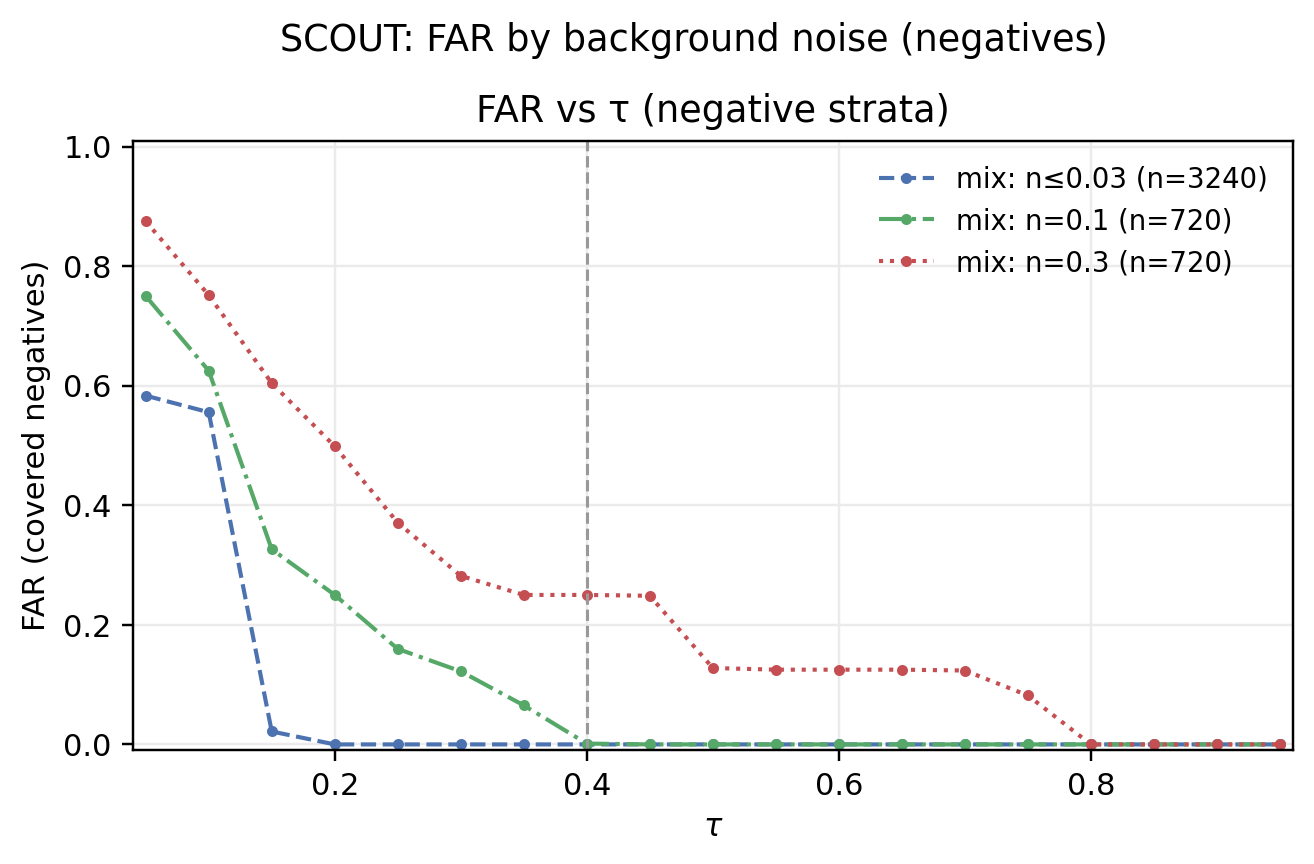
\includegraphics[width=0.9\linewidth]{figures/exp22v2_scout_far_by_noiseprob_minT64.png}
\caption{FAR stratified by noise coverage $n$. Only the $n=0.3$ subset (approximately 30\% of segments containing background noise) contributes nearly all of the FAR; the FAR of all other subsets is close to zero.}
\label{fig:c5-a7}
\end{figure}

%Figure~\ref{fig:c5-gating-mask-overlap} overlays the gating trigger region onto the triage heatmap: the gating mask primarily covers regions where triage cost has already inflated significantly or entered N/A, while it almost never triggers in low-cost regions; the trigger boundary exhibits a sharp transition (Figure~\ref{fig:c5-gating-boundary}), indicating that the gating signal is spatially aligned with the degradation region of triage.

% \begin{figure*}[!thbp]
% \centering
% \begin{minipage}[c]{0.64\linewidth}
%   \centering
%   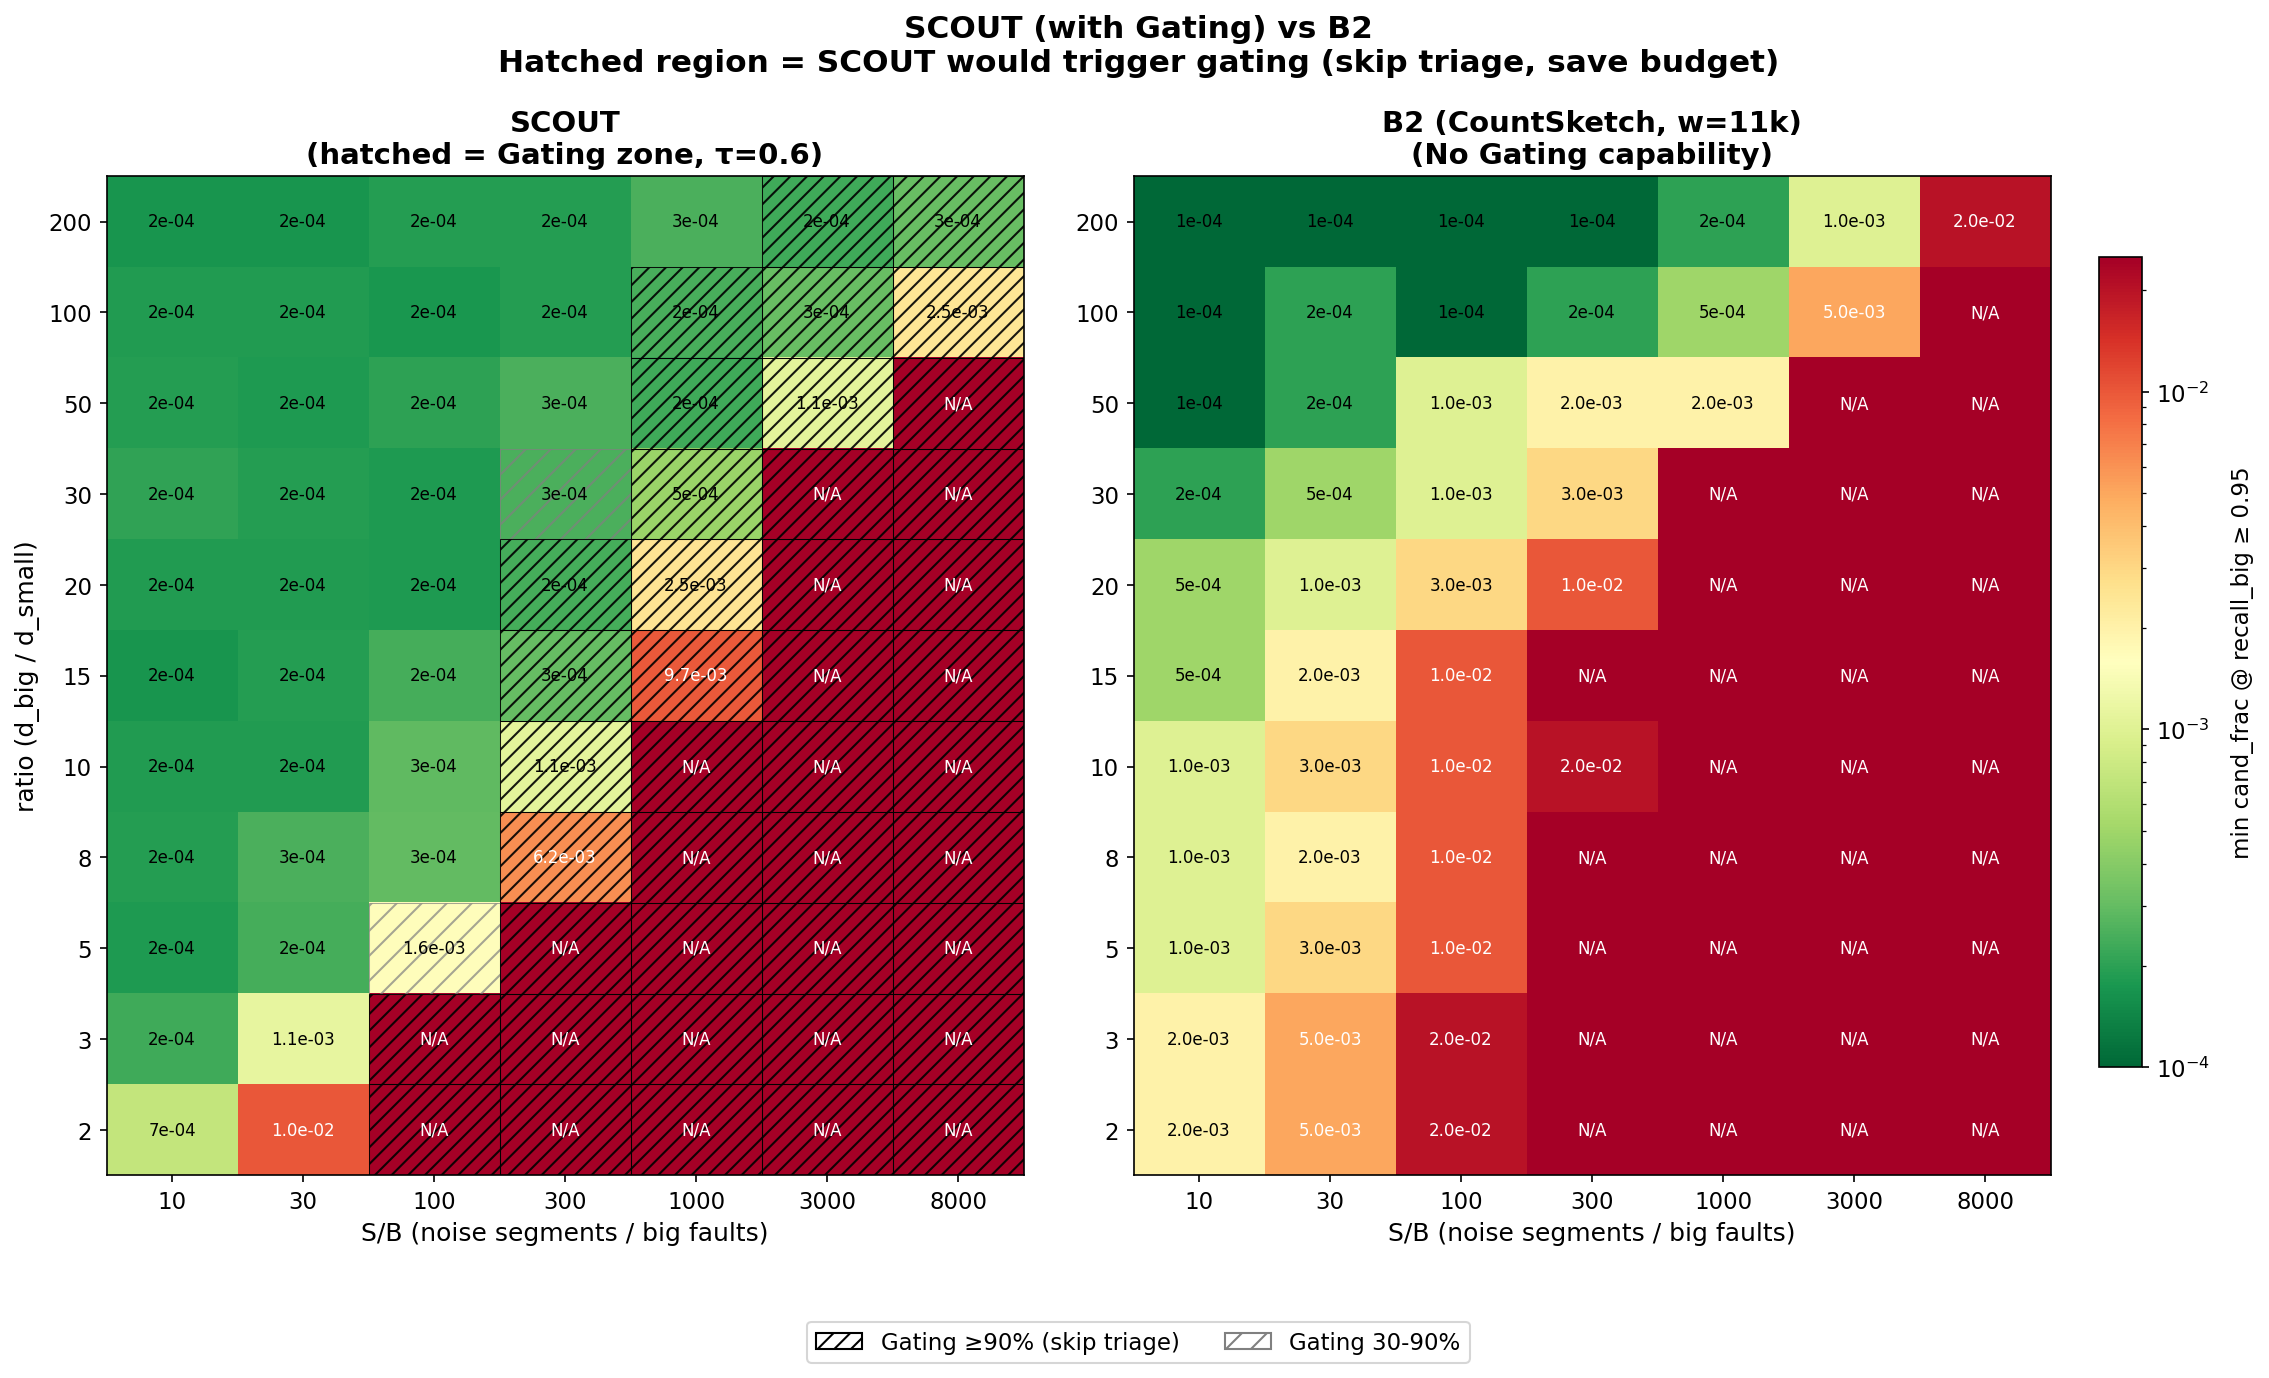
\includegraphics[width=\linewidth]{figures/exp20v4_scout_gating_vs_b2.png}
%   \subcaption{SCOUT's gating mask (hatched region) overlaid on the triage threshold-budget heatmap (left); B2's triage heatmap (right) is shown for reference---B2 has no comparable gating mechanism.}
%   \label{fig:c5-gating-mask-overlap}
% \end{minipage}\hfill
% \begin{minipage}[c]{0.32\linewidth}
%   \centering
%   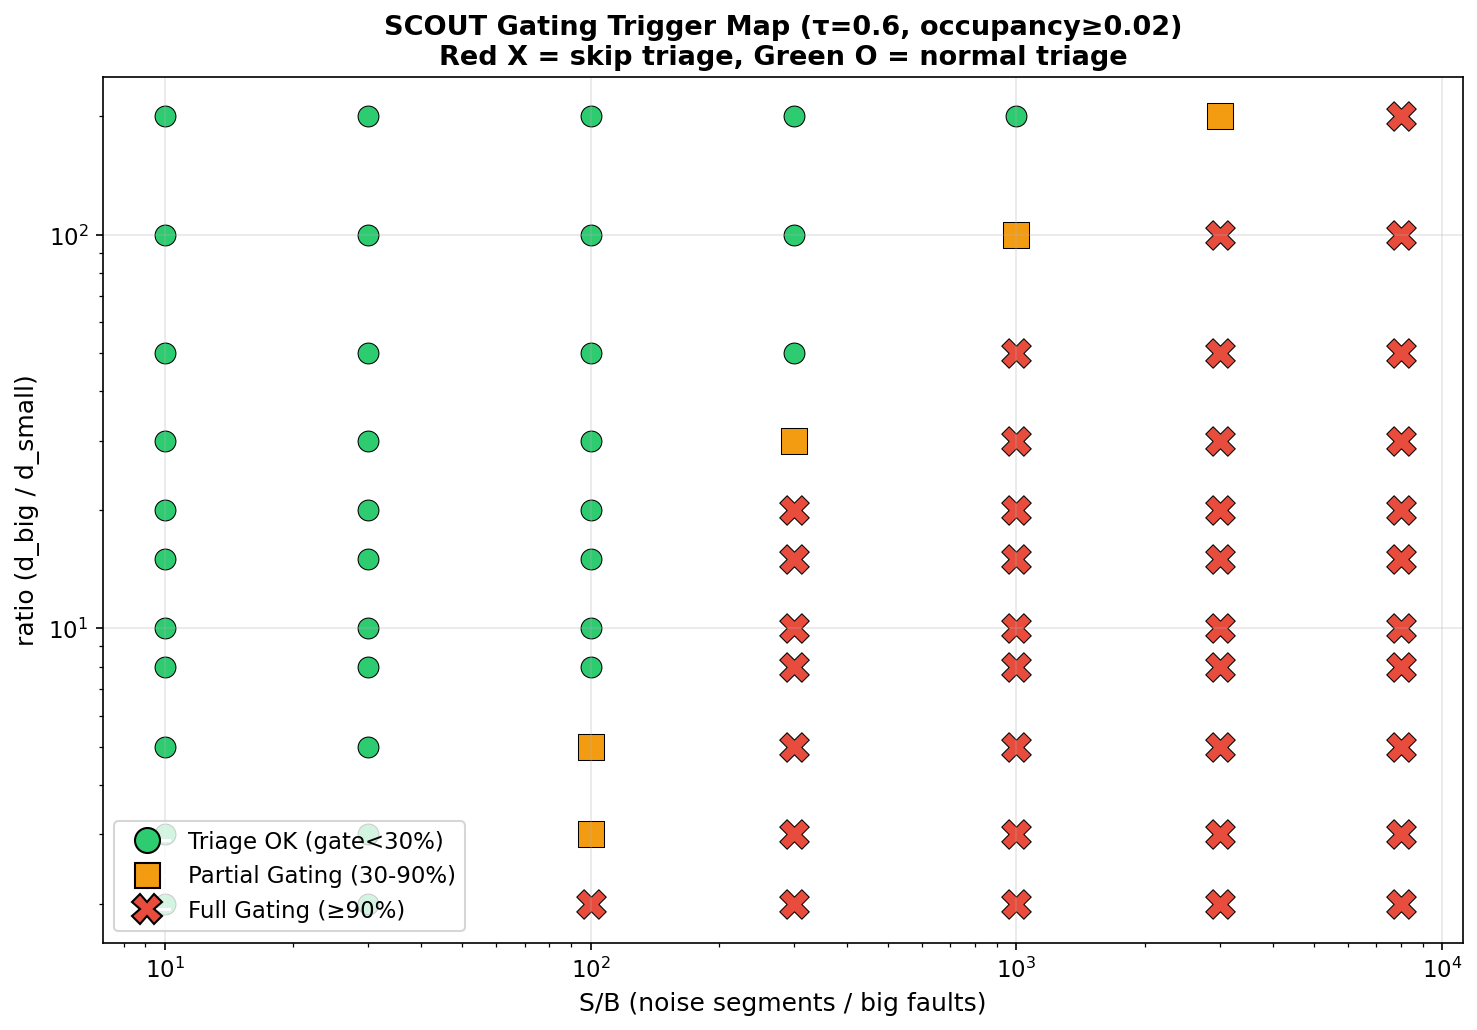
\includegraphics[width=\linewidth]{figures/exp20v4_gating_boundary.png}
%   \subcaption{Gating trigger boundary of SCOUT. The transition from ``normal triage'' to ``full gating'' is sharp, with the boundary approximately along $\texttt{S/B}\approx 100$--300.}
%   \label{fig:c5-gating-boundary}
% \end{minipage}
% \caption{Gating mask and trigger boundary.}
% \end{figure*}

\begin{table}[!thbp]
\centering
\small
\begin{tabular}{lrccc}
\toprule
Method & $\tau_{\text{gating}}$ & \texttt{FAR\_cond} & \texttt{FRR\_cond} & \texttt{decisive (neg)} \\
\midrule
SCOUT & 0.30 & 0.062 & 0.10 & 0.93 \\
SCOUT & 0.35 & 0.049 & 0.10 & 0.93 \\
SCOUT & \textbf{0.40} & \textbf{0.039} & \textbf{0.10} & 0.93 \\
SCOUT & 0.45 & 0.038 & 0.34 & 0.93 \\
B2 & 0.05 & \textbf{0.47} & 0.25 & 1.0 \\
B2 & 0.15 & 0.43 & \textbf{0.50} & 1.0 \\
B2 & 0.35 & 0.34 & \textbf{0.50} & 1.0 \\
B2 & 0.80 & 0.07 & \textbf{0.50} & 1.0 \\
B2 & 0.90 & 0.00 & 0.75 & 1.0 \\
B3 & 0.50 & \textbf{1.00} & 0.00 & 0.875 \\
B3 & 0.65 & \textbf{0.99} & 0.09 & 0.875 \\
B3 & 0.70 & \textbf{0.96} & 0.33 & 0.875 \\
B3 & 0.85 & 0.36 & 0.93 & 0.875 \\
B3 & 0.95 & 0.02 & 1.00 & 0.875 \\
\bottomrule
\end{tabular}
\caption{Complete threshold sweep for the $\sim$768\,KiB control setting (\texttt{min\_touched=64}). The table reports conditional false-alarm rate \texttt{FAR\_cond}, conditional false-reject rate \texttt{FRR\_cond}, and \texttt{decisive (neg)}. Here, \texttt{decisive (neg)} denotes the fraction of negative-class samples that receive a decisive (non-\texttt{unknown}) classification; the negative class corresponds to bimodal/mix samples, since \texttt{gate} is treated as the positive class.}
\label{tab:c5-1}
\end{table}

\subsubsection{\texttt{unknown} Fraction Does Not Affect Conclusions}

For gating, the main text reports $\mathrm{FAR_{cond}}$ and
$\mathrm{FRR_{cond}}$ over decisive samples, excluding samples
labeled \texttt{unknown}. Supplement Table~\ref{tab:c5-1}
therefore reports \texttt{decisive (neg)}, the fraction of
negative-class samples that receive a decisive rather than
\texttt{unknown} classification. The reported values are 0.93
for SCOUT, 1.0 for B2, and 0.875 for B3, which correspond to
approximately 7\%, 0\%, and 12.5\% \texttt{unknown},
respectively. These exclusion rates are modest and do not
account for the observed errors: B2 still reaches
$\mathrm{FAR_{cond}}=0.47$ with 100\% decisive classifications,
and B3 remains near $\mathrm{FAR_{cond}}=1.0$ at
$\tau_{\text{gating}}=0.50$. The failures therefore reflect
insufficient discriminability rather than the exclusion of
difficult samples as \texttt{unknown}.
